\section{Theorie}
\label{sec:theorie}

    Im Folgenden sollen die theoretischen Grundlagen der Untersuchung des Compton-Effekts erläutert werden.\\
    \\
    Der Compton-Effekt zeigt,
    dass sich die Wellenlänge von $\gamma$-Strahlung bei Streuung an einem Elektron verändert.
    Um dies zu untersuchen,
    werden die Streuung von Röntgenstrahlung an einem Plexiglasquader
    sowie das Transmissions- und Absorptionsverhalten beobachtet.

\subsection{Entstehung und Eigenschaften von Röntgenstrahlung}
\label{sec:röntgen}

    Zur Erzeugung von Röntgenstrahlung wird eine evakuierte Röntgenröhre verwendet.
    In dieser werden mithilfe einer negativ geladenen Glühkathode freie Elektronen erzeugt
    und zu einer positiv geladenen Anode hin beschleunigt.
    Beim Auftreffen der Elektronen auf die Anode werden sie im Coloumbfeld der Anodenatome abgebremst,
    wobei die Elektronen einen Teil ihrer Energie in Form eines Photons abgeben.
    Das entstehende Bremsspektrum ist kontinuierlich,
    da die Elektronen unterschiedlich viel Energie abgeben
    und einen Teil ihrer kinetischen Energie zurückbehalten können.
    Zudem ionisieren die Elektronen die Atome des Anodenmaterials,
    sodass diese ihrerseits auch Photonen emittieren,
    welche jedoch eine diskrete Energie,
    der Energiedifferenz der Atomschalen entsprechend,
    besitzen.
    Es entstehen Peaks,
    deren Energie charakteristisch für das verwendete Anodenmaterial ist.\\
    \\
    Die Transmission eines Stoffes ist abhängig von der Wellenlänge und nimmt mit zunehmender Wellenlänge ab.\\
    Die Absorption nimmt dementsprechend mit der Wellenlänge zu.
    Der Verlauf der Absorption in Abhängigkeit der Dicke des Materials wird durch das Delamber'sche Gesetz beschrieben.
    Dieses besagt
    \begin{equation}
        I = I_0 \cdot \exp{(-\mu d)} \ ,
    \end{equation}
    wobei $I_0$ die einfallende Intensität darstellt.
    Da bei Röntgenstrahlung die dominierenden Prozesse der Photoeffekt,
    die Paarbildung und der hier untersuchte Compton-Effekt sind,
    setzt sich der Absorptionskoeffizient aus
    \begin{equation*}
        \mu = \mu_\text{Photo} + \mu_\text{Paar} + \mu_\text{Com}
    \end{equation*}
    zusammen,
    mit den entsprechenden Absorptionskoeffizienten dieser Effekte.\\
    \\
    Mithilfe der Bragg-Reflexion kann die Wellenlänge der Röntgenstrahlung untersucht werden.
    \begin{figure}[H]
       \centering
        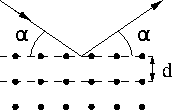
\includegraphics[width=0.25\textwidth]{content/img/Abb_nonumber_bragg.pdf}
        \caption{Reflexion der Röntgenstrahlung an einem Gitterkristall. \cite{versuchsanleitung}}
       \label{fig:bragg_reflexion}
    \end{figure}
    Die Röntgenstrahlung wird an einem Gitterkristall gebeugt,
    wie in \autoref{fig:bragg_reflexion} dargestellt,
    wobei die Strahlen bei einem Glanzwinkel $\alpha$ konstruktiv interferieren
    und die gebeugte Wellenlänge in der Beugungsordnung $n$
    mithilfe der Bragg-Bedingung
    \begin{equation}
        2d \sin{\alpha} = n \lambda
        \label{eqn:bragg_bedingung}
    \end{equation}
    berechnet werden kann.


\subsection{Der Compton-Effekt}
\label{sec:compton_effekt}

    Zur Untersuchung des Compton-Effekts wird nun die Röntgenstrahlung an einem Plexiglasquader gestreut.
    Dabei kann sowohl kohärente, also inelastische Streuung,
    als auch inkohärente, also elastische Streuung,
    auftreten.
    Bei der inkohärenten Streuung stößt ein Photon mit einem Elektron zusammen und wird unter Abgabe von Energie um den Winkel $\alpha$ gestreut.
    Sowohl Photon als auch Elektron verändern dabei ihre Bewegungsrichtung.
    Dies wird in \autoref{fig:compton} dargestellt.
    \begin{figure}[H]
        \centering
        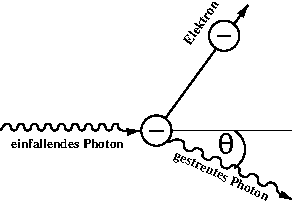
\includegraphics[width=0.6\textwidth]{content/img/Abb_1.pdf}
        \caption{Der Compton-Effekt: Streuung eines Photons an einem Elektron. \cite{versuchsanleitung}}
        \label{fig:compton}
    \end{figure}
    Durch die Energieabgabe verändert sich die Wellenlänge des Photons
    um eine Wellenlängendifferenz
    \begin{equation}
        \symup{\Delta}\lambda = \lambda_2 - \lambda_1
        \label{eqn:wellenlängendifferenz}
    \end{equation}
    mit der ungestreuten Wellenlänge $\lambda_1$ und der verlängerten Wellenlänge $\lambda_2$ nach der Streuung.

    Aus der Energie- und Impulserhaltung bei der Streuung kann außerdem die Beziehung
    \begin{equation}
        \symup{\Delta}\lambda = \frac{h}{m_\text{e} c}(1 - \cos{\theta})
        \label{eqn:verschiebung_winkelabhängig}
    \end{equation}
    hergeleitet werden,
    wobei der Faktor $\lambda_\text{c} = \sfrac{h}{m_\text{e}c}$ die konstante Compton-Wellenlänge des Elektrons beschreibt.
    %Sie kann mithilfe der Gleichungen \ref{eqn:wellenlängendifferenz} und \ref{eqn:verschiebung_winkelabhängig} durch
    %\begin{equation}
    %    \lambda_\text{c} = \frac{h}{m_\text{e}c} = \frac{\lambda_2 - \lambda_1}{1 - \cos{\alpha}}
    %    \label{eqn:compton_wellenlänge}
    %\end{equation}
    %berechnet werden.
    Abhängig vom Streuwinkel verändert sich die Wellenlängenverschiebung bei der Streuung.
    Bei $\theta = \SI{0}{\degree}$ ist die Verschiebung mit $\symup{\Delta}\lambda = 0$ minimal und
    bei $\theta = \SI{180}{\degree}$ ist die Verschiebung mit $\symup{\Delta}\lambda = 2\lambda_\text{c}$ maximal.
